\section{Détection de contours et extraction de lignes}

\subsection{Détection de contours}

La première étape de notre processus de reconnaissance de grillage est de détecter les contours d'une image. En effet, les grillages provoquent naturellement une notion de contours dans l'image de par leur superposition sur le paysage.

Il existe de nombreuses manières d'obtenir un détecteur de contours, nous avons opté pour la méthode de Canny. Celle-ci a l'avantage de procéder par seuillage par hysteresis ce qui permet d'obtenir de bons résultats - au prix d'une recherche des paramètres optimaux. A COMPLETER.

\begin{figure}[ht!]
\centering
\begin{tabular}{cc}
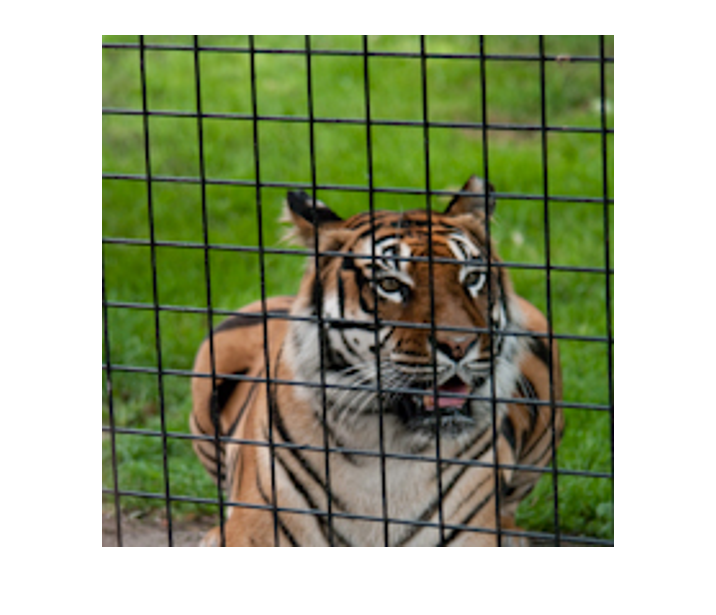
\includegraphics[width = .5\columnwidth]{fig/tigre_rescale.png} &
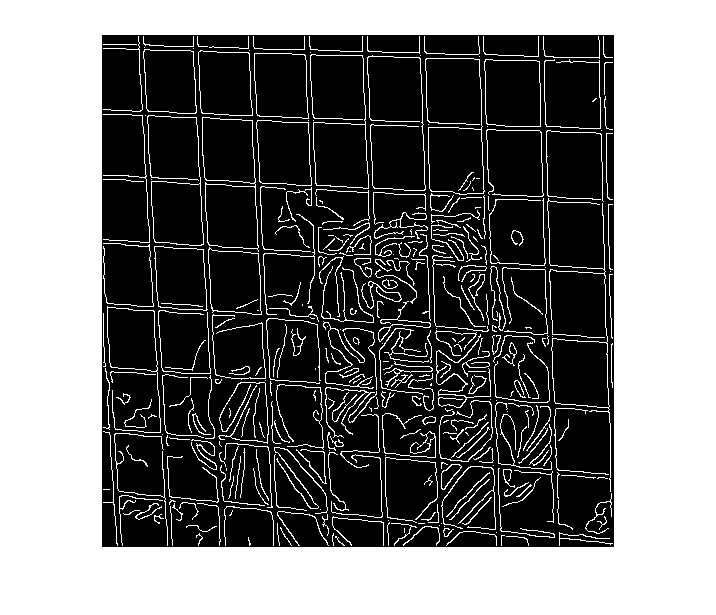
\includegraphics[width = .5\columnwidth]{fig/contour.png} \\
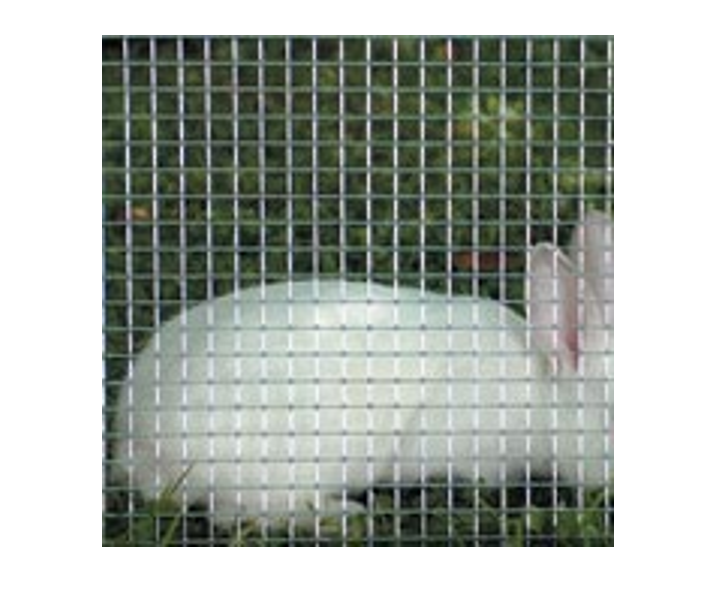
\includegraphics[width = .5\columnwidth]{fig/lapin_rescale.png} &
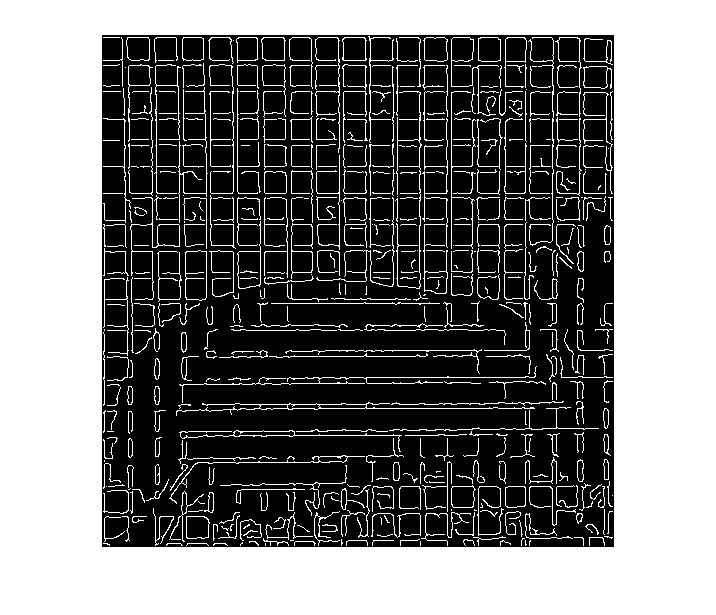
\includegraphics[width = .5\columnwidth]{fig/contour_lapin.png} \\
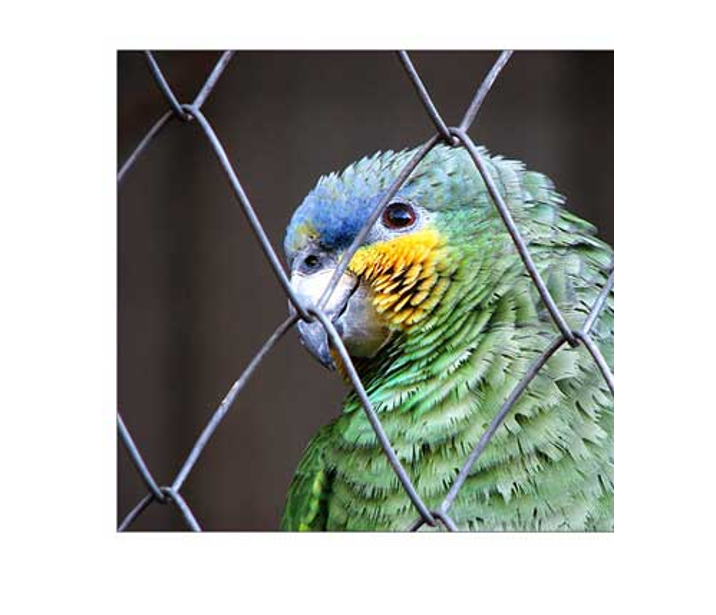
\includegraphics[width = .5\columnwidth]{fig/parrot_rescale.png} &
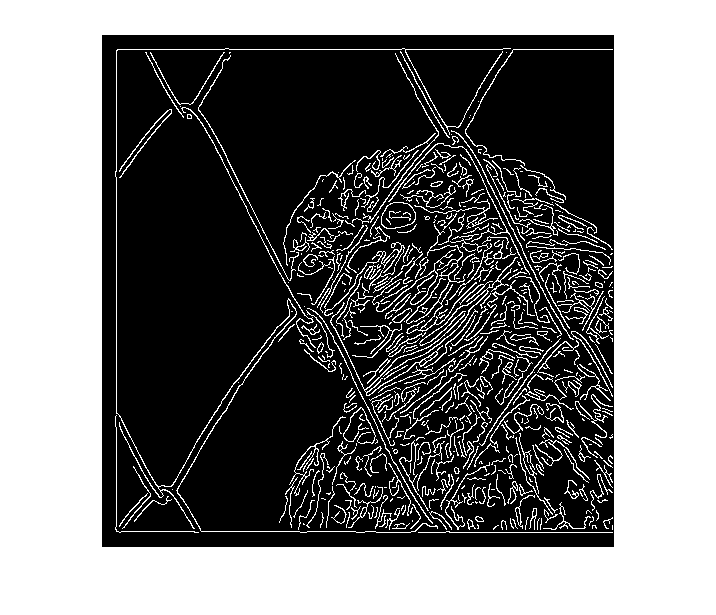
\includegraphics[width = .5\columnwidth]{fig/contour_parrot.png}
\end{tabular}
\caption{Dans les colonnes de gauche, l'image initiale et dans celles de droite les résultats de la détection de contour avec l'algorithme de Canny. Toutes les images sont redimensionnées en $512\times 512$. }
\end{figure}

\subsection{Extraction de lignes - transformation de Hough}

A ECRIRE.
